\section{Gesamtarchitektur}

\setauthor{\firstauthor}
\section{Multi-Step-Funnel}
\subsection{Erstellung der Website}
%Erwähnen, dass Impressum, Datenschutz etc auch vorhanden sind.
Die Website wurde mit dem No-Code-Tool \textit{Framer} erstellt. 
Dieses bietet eine benutzerfreundliche Oberfläche zur Gestaltung 
von interaktiven Webseiten.

\subsubsection{Design der Website}
Zu Beginn wurden die grundlegenden Seitenstrukturen und das Design
festgelegt. Dabei wurde sich in erster Linie an die
Corporate Identity der App gehalten.
Diese beinhaltet insbesondere:
\begin{itemize}
    \item Farbpalette
    \item Schriftarten
    \item Logo
    \item Stark abgerundete Buttons und Formen
\end{itemize}

Die grundlegende Farbpalette besteht aus den in Abbildung \ref{fig:impl:companycolors} 
dargestellten Farben. 
Diese wurden sowohl für die Gestaltung der Landingpage als auch 
der Funnel-Seiten verwendet, um ein konsistentes Erscheinungsbild 
zu gewährleisten.
Die Farben finden sich in Buttons, Schriften, Hintergründen und anderen 
Designelementen wieder.

\begin{figure}[H]
    \centering
    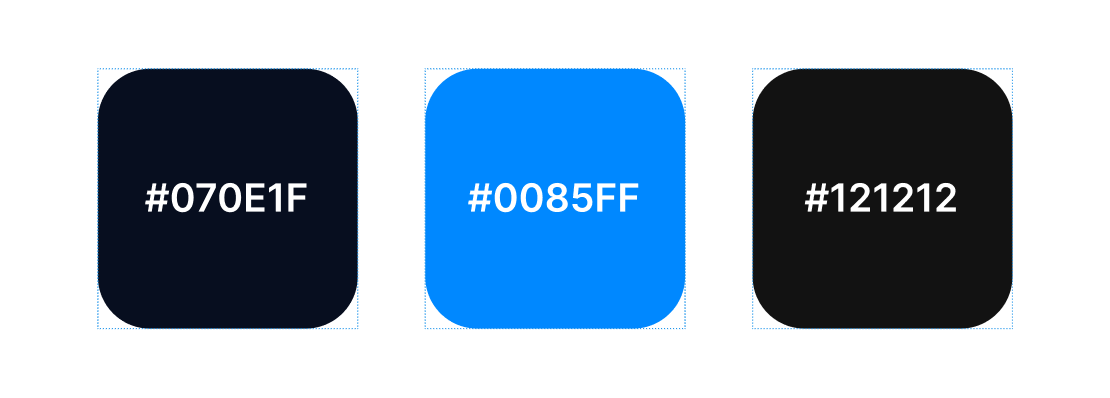
\includegraphics[scale=0.3]{pics/company-colors.png}
    \caption{Farbpalette des Unternehmens}
    \label{fig:impl:companycolors}
\end{figure}

Weiters wurde ausschließlich die Schriftart \textit{Inter} verwendet,
da diese Teil der Corporate Identity der App ist.
Inter ist eine moderne, serifenlose Schriftart, die sich durch eine gute 
Lesbarkeit auszeichnet und sich daher besonders für digitale Anwendungen eignet.
Die verwendete Schriftart ist in Abbildung \ref{fig:impl:inter} dargestellt.

\begin{figure}[H]
    \centering
    
\includegraphics[scale=0.5]{pics/inter-font.png}
    \caption{Schriftart Inter - Corporate Font der App}
    \label{fig:impl:inter}
\end{figure}

Serifenlose Schriftarten sind besonders gut für dunkle Hintergründe auf
Websites geeignet, da die klaren Linien und das Fehlen von Serifen die 
Lesbarkeit verbessern. Serifenlose Schriften sind zwar nicht zwingend ästhetisch
ansprechender als serifenbehaftete Schriftarten, jedoch auf Bildschirmen
besser lesbar, was die Nutzererfahrung positiv beeinflusst.
\cite{SerifVSSansSerifUXImpact2026}

Außerdem wurden deutlich abgerundete Buttons und Formen verwendet, 
um ein modernes und freundliches Design zu schaffen.

Wichtige Kennzahlen und Überschriften wurden durch die Verwendung von 
größeren Schriftgrößen und Schriftstärken hervorgehoben.
Große präsente Texte ziehen die Aufmerksamkeit der Nutzer:innen auf 
sich und vermitteln die wichtigsten Informationen auf einen Blick.

\subsubsection{Erstellung der Landingpage}
Auf der Landingpage wurde der zentrale Text mit einer Schriftgröße von 
\textit{70pt} und einer Schriftstärke von \textit{700} gestaltet, um den 
Nutzer:innen bereits zu Beginn klar zu vermitteln, worum es auf der Website geht.
Darunter befindet sich eine etwas kleinere Unterüberschrift
mit derselben Schriftstärke und einer Größe von \textit{40pt}, 
die weitere Informationen zum Angebot der App liefert.

Auf der Landingpage befindet sich außerdem ein zentral platzierter Button mit der Aufschrift
„Jetzt entdecken“. Dieser fungiert als klarer Call-to-Action und 
ermutigt die Nutzer:innen, den Funnel zu starten.

Im unteren Bereich der Startseite werden, wie in Abbildung 
\ref{fig:impl:landingpage} dargestellt,
Logos von Unternehmen präsentiert, die dem Unternehmen bereits vertrauen
und die App bereits zum Zeitpunkt des Launches einsetzen werden.
Dadurch wird bereits zu Beginn Vertrauen aufgebaut und die Glaubwürdigkeit 
der App gestärkt.

Die Logos bewegen sich dabei in einer Endlosschleife von rechts nach links 
über die Seite, wodurch zusätzliche Aufmerksamkeit erzeugt und das Interesse 
der Nutzer:innen weiter gesteigert wird.
Dieses dynamische Element heißt in \textit{Framer} "Ticker"
und ist eine einfache Möglichkeit, um Bewegung und Dynamik auf 
der Seite zu erzeugen.

Zusätzlich wurde bei der Gestaltung der Landingpage auf eine klare visuelle Hierarchie geachtet. 
Durch die Verwendung unterschiedlicher Schriftgrößen wird der Blick der Nutzer:innen gezielt 
vom Haupttitel über die Unterüberschrift bis hin zum Call-to-Action geleitet. Dadurch wird sichergestellt, 
dass die wichtigsten Informationen zuerst wahrgenommen werden.

Die gesamte Gestaltung der Landingpage ist bewusst minimalistisch gehalten, um Ablenkungen zu vermeiden 
und den Fokus auf die zentrale Botschaft der App zu legen. Auf zusätzliche Navigationselemente oder 
überflüssige Inhalte wurde verzichtet, um die Nutzer:innen möglichst direkt zum nächsten Schritt im 
Funnel zu führen.

Das Layout ist zentral ausgerichtet, wodurch eine klare und strukturierte Darstellung 
entsteht. Diese Zentrierung unterstützt die visuelle Führung und sorgt dafür, dass alle wichtigen Inhalte 
im direkten Blickfeld der Nutzer:innen liegen.

Besonderes Augenmerk wurde auch auf das Farbkonzept gelegt. Der dunkle Hintergrund erzeugt einen hohen 
Kontrast zu den hellen Texten und dem farblich hervorgehobenen Call-to-Action-Button. Dadurch wird die 
Lesbarkeit verbessert und gleichzeitig sichergestellt, dass interaktive Elemente sofort erkannt werden.

Da die Landingpage den ersten Kontaktpunkt mit der App darstellt, wurde sie nach dem sogenannten 
\textit{Above-the-Fold}-Prinzip gestaltet. Das bedeutet, dass alle entscheidenden Informationen sowie der 
Call-to-Action ohne Scrollen sichtbar sind. Dadurch wird sichergestellt, dass Nutzer:innen unmittelbar 
verstehen, worum es geht und welche Handlung von ihnen erwartet wird.

\begin{figure}[H]
    \centering
    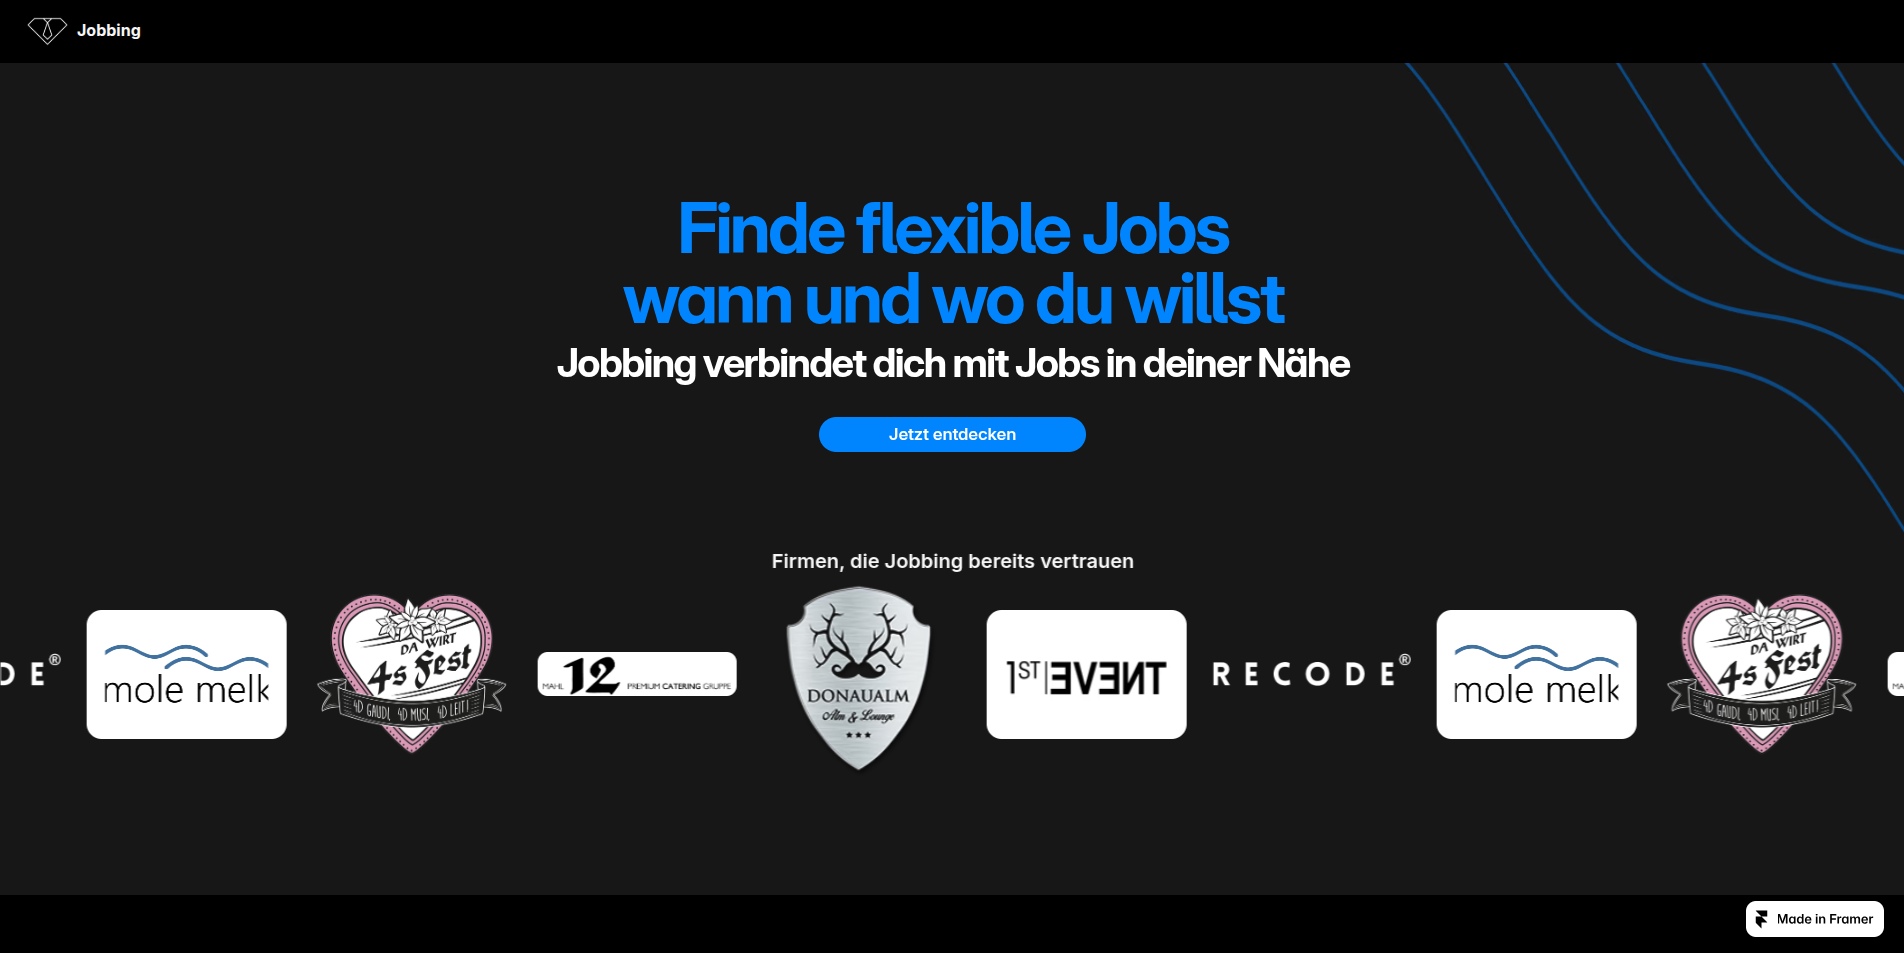
\includegraphics[scale=0.2]{pics/landing-page.png}
    \caption{Landingpage der Website - Desktop-Version}
    \label{fig:impl:landingpage}
\end{figure}

\subsubsection{Erstellung der Funnel-Seiten}
\subsubsection{Responsiveness}
\subsubsection{Probleme bei der Erstellung}

\setauthor{\secondauthor}
\section{Chatbot}

\setauthor{\firstauthor}
\section{Hosting}

\setauthor{\firstauthor}
\section{Datenerfassung}
\subsection{Framer Analytics}

\subsection{Implementierung von Google Analytics}
\begin{lstlisting}[
    language=HTML,
    caption=Code zur Implementierung von Google Analytics,
    label=lst:impl:googleanalyticsimplementation
]
<!-- Google tag (gtag.js) -->
<!-- ########## muss durch die eigene Tracking-ID ersetzt werden -->
<script async src="https://www.googletagmanager.com/gtag/js?id=G-##########"></script>
<script>
  window.dataLayer = window.dataLayer || [];
  function gtag(){dataLayer.push(arguments);}
  gtag('js', new Date());

  gtag('config', 'G-##########');
</script>
\end{lstlisting}

\subsection{Implementierung von Microsoft Clarity}
\begin{lstlisting}[
    language=HTML,
    caption=Code zur Implementierung von Microsoft Clarity,
    label=lst:impl:microsoftclarityimplementation
]
<!-- ########## muss durch die eigene Tracking-ID ersetzt werden -->
<script type="text/javascript">
    (function(c,l,a,r,i,t,y){
        c[a]=c[a]||function(){(c[a].q=c[a].q||[]).push(arguments)};
        t=l.createElement(r);t.async=1;t.src="https://www.clarity.ms/tag/"+i;
        y=l.getElementsByTagName(r)[0];y.parentNode.insertBefore(t,y);
    })(window, document, "clarity", "script", "##########");
</script>
\end{lstlisting}

\subsection{Erstellung des Google Forms}


\section{Backend}

\section{Datenvisualisierung}


Siehe tolle Daten in Tab. \ref{tab:impl:data}.

%\begin{table}
%    \centering
%    \begin{tabular}{|lcc|}
%    \hline
%              & \textbf{Regular Customers} & \textbf{Random Customers} \\ \hline
%    Age       & 20-40                      & \textgreater{}60          \\ \hline
%    Education & university                 & high school               \\ \hline
%    \end{tabular}
%    \caption{Ein paar tabellarische Daten}
%    \label{tab:impl:data}
%\end{table}

%\begin{figure}
%    \centering
 %   
\includegraphics[scale=0.5]{pics/knuthi.jpg}
  %  \caption{Don Knuth -- CS Allfather}
   % \label{fig:impl:knuth}
%\end{figure}

Siehe und staune in Abb. \ref{fig:impl:knuth}.
Dann betrachte den Code in Listing \ref{lst:impl:foo}.

%\begin{lstlisting}[language=Python,caption=Some code,label=lst:impl:foo]
%# Program to find the sum of all numbers stored in a list (the not-Pythonic-way)

%# List of numbers
%numbers = [6, 5, 3, 8, 4, 2, 5, 4, 11]

%# variable to store the sum
%sum = 0

%# iterate over the list
%for val in numbers:
%    sum = sum+val

%print("The sum is", sum)
%\end{lstlisting}